\subsection{Simulación con LTSpice}

Se simula el circuito de la fig. \ref{fig:1:esquema} con LTSpice buscando el 
punto de operación (\verb|.op|), como puede verse en la captura de pantalla
de la fig. \ref{fig:1:ltspice}. Los datos obtenidos se encuentran en las tablas
\ref{tab:1:ltspice-tensiones} y \ref{tab:1:ltspice-corrientes}.

Tomando los valores de la tabla \ref{tab:1:ltspice-tensiones} se llega,
mediante la ec. \ref{ec:1-teoria:ganancia}, a un valor de $A = 1.517$ para
todos los casos. Dicho valor concuerda con el análisis teórico de la sección
anterior, aunque su incertidumbre es difícil de estimar.

\begin{figure}[H]
    \centering
    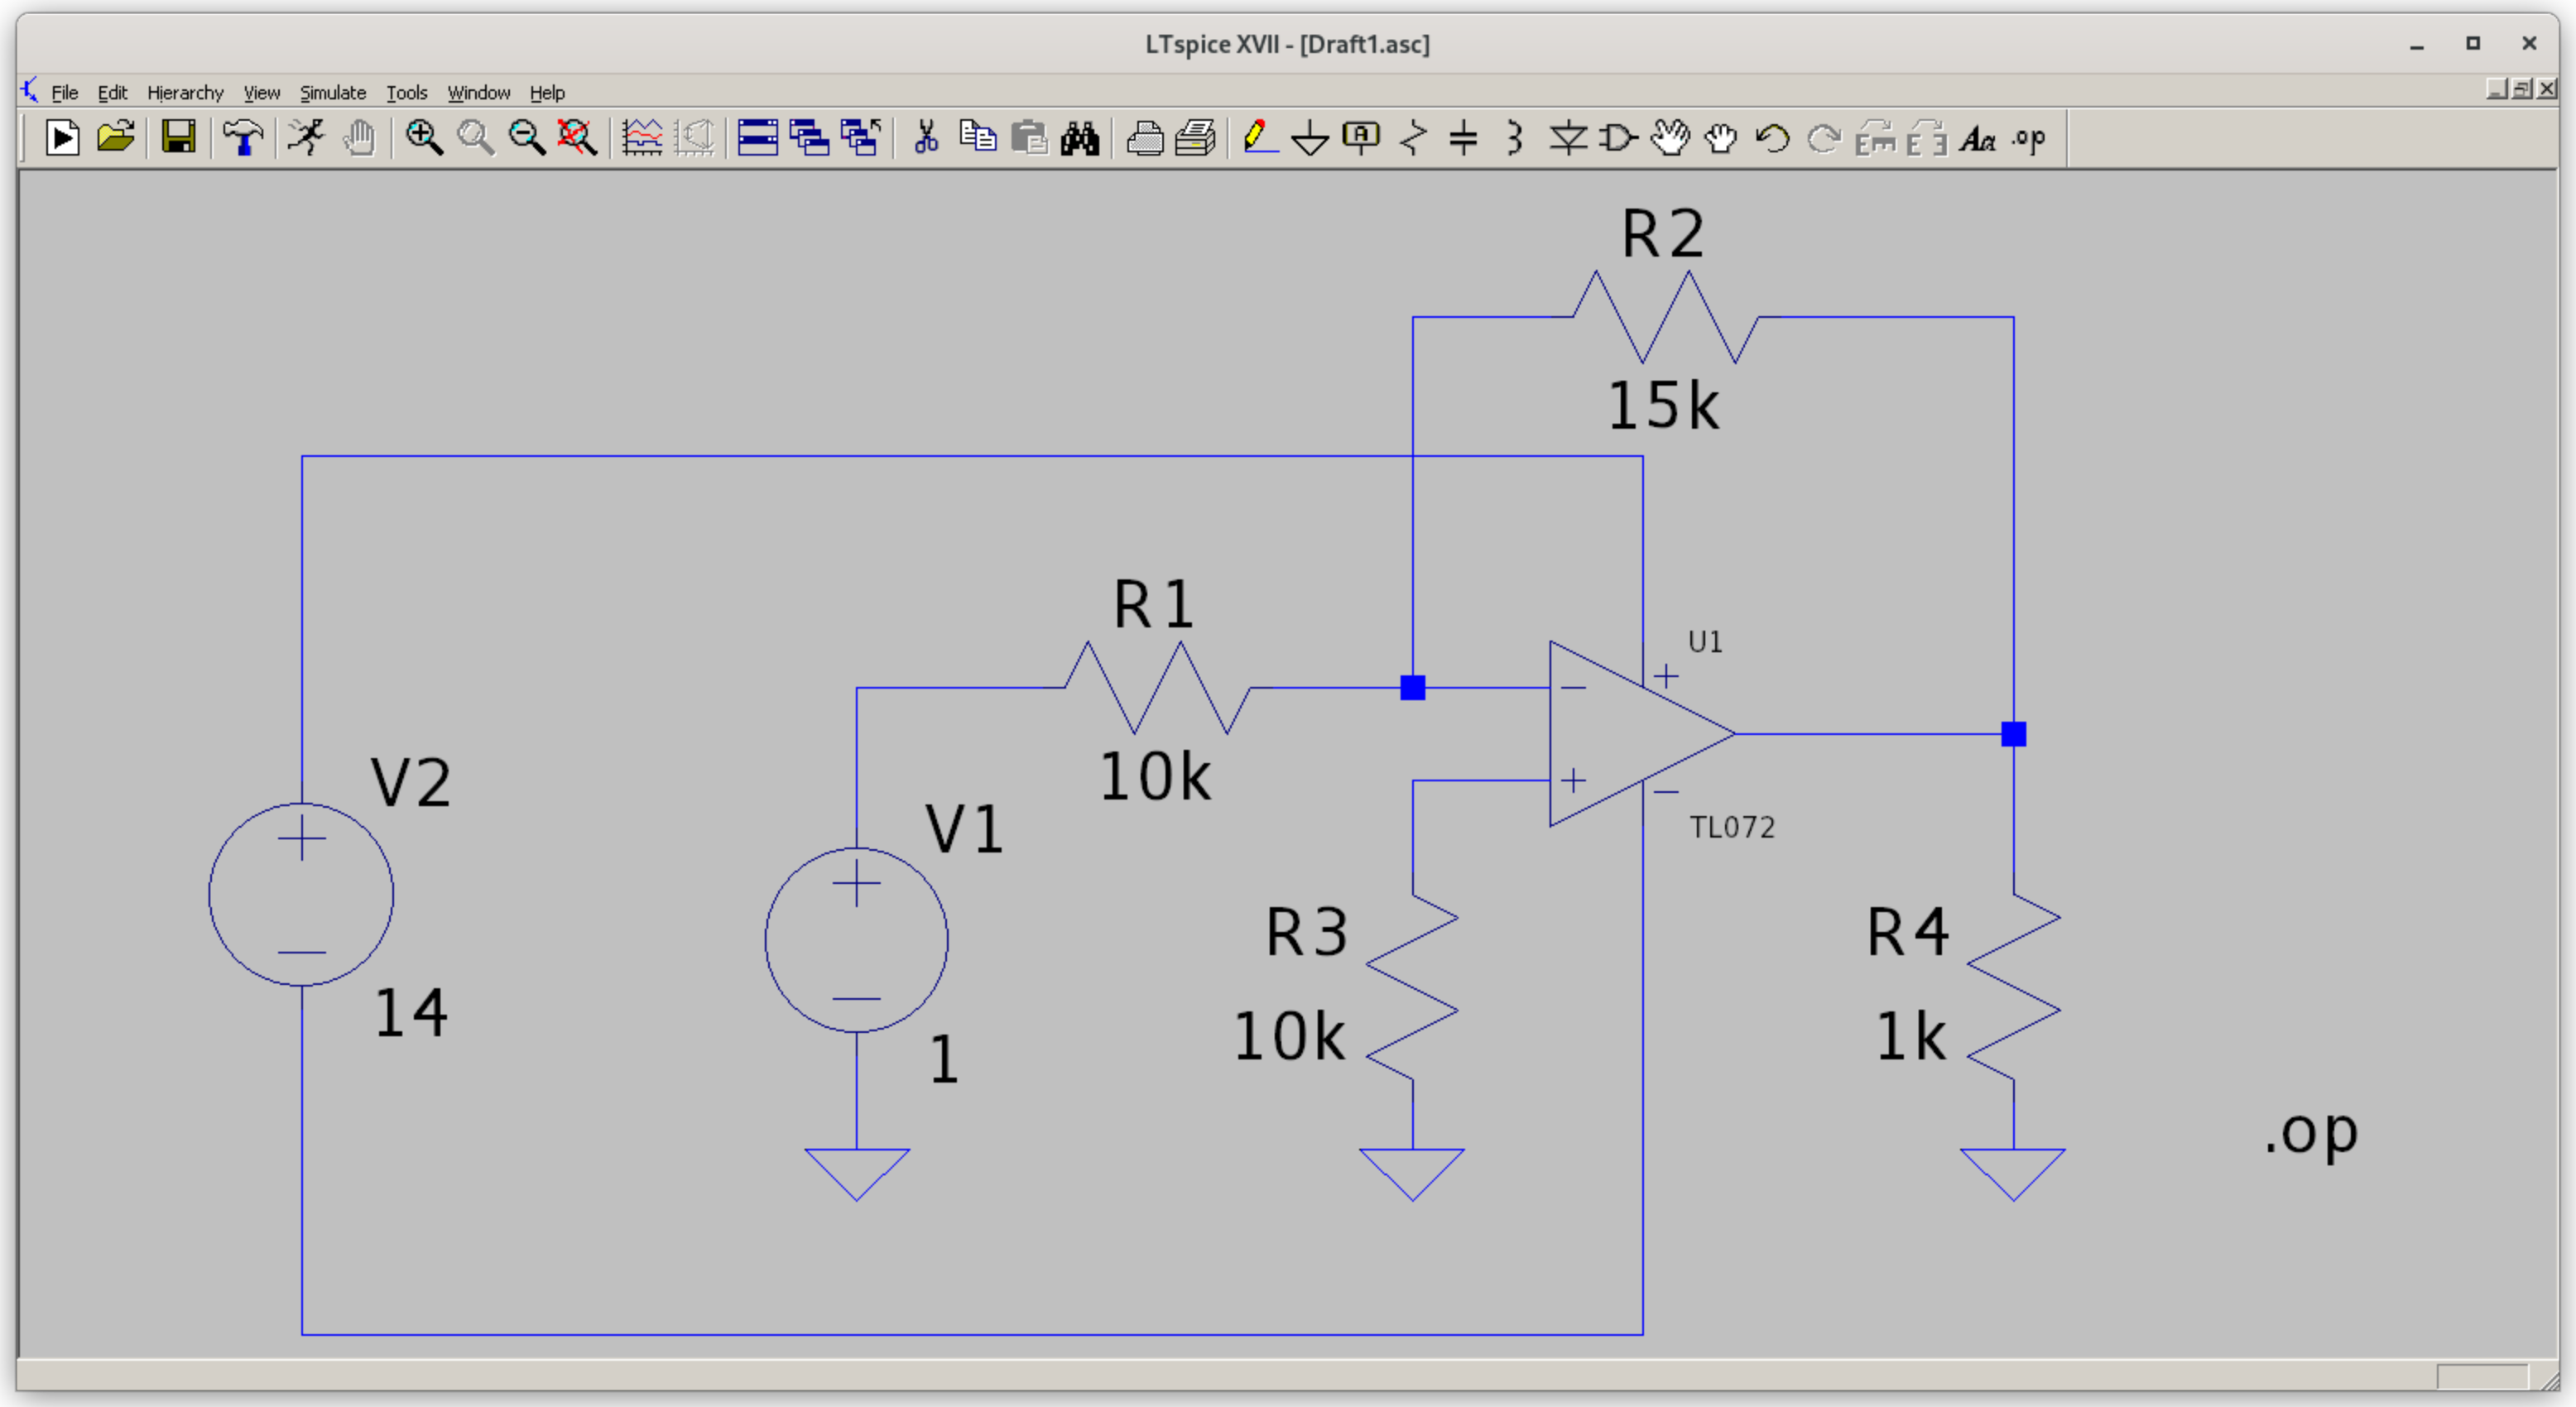
\includegraphics[width=0.8\textwidth]{img/1/ltspice.png}
    \caption{Pantalla de LTSpice}
    \label{fig:1:ltspice}
\end{figure}

\begin{table}[H]
    \centering
    \begin{tabular}{@{}r|rrrr@{}}
    \toprule
    $R_L$ (\si{\kilo\ohm}) & $v_o$ (\si{\volt}) & $v_+$ (\si{\nano\volt}) & 
    $v_-$ (\si{\milli\volt}) & $v_+ - v_-$ (\si{\milli\volt}) \\
    \midrule
    $47$ & $-13.6573$ & $-562.558$ & $-62.9007$ & $62.9001$ \\
    $10$ & $-13.5672$ & $-562.558$ & $-62.8992$ & $62.8986$ \\
     $1$ & $-13.6572$ & $-562.557$ & $-62.8821$ & $62.8815$ \\ \bottomrule
    \end{tabular}
    \caption{Tensiones según LTSpice ($v_i = \SI{9.00}{\volt}$)}
    \label{tab:1:ltspice-tensiones}
\end{table}

\begin{table}[H]
    \centering
    \begin{tabular}{@{}r|rrrr@{}}
        \toprule
        $R_L$ (\si{\kilo\ohm}) & $I_{R_1}$ (\si{\milli\ampere}) &
        $I_{R_2}$ (\si{\milli\ampere}) & $I_{R_3}$ (\si{\pico\ampere}) &
        $I_{R_L}$ (\si{\milli\ampere}) \\
        \midrule
        $47$ & $0.29058$ & $0.906290$ & $56.2558$ & $0.29058$ \\
        $10$ & $1.36572$ & $0.906290$ & $56.2558$ & $1.36572$ \\
         $1$ & $13.6572$ & $0.906288$ & $56.2557$ & $13.6572$ \\ \bottomrule
        \end{tabular}
        \caption{Corrientes según LTSpice}
        \label{tab:1:ltspice-corrientes}
\end{table}

